\documentclass[tikz,border=0pt]{standalone}
\usepackage[utf8]{inputenc}
\usepackage{xcolor}

\newcommand{\cardwidth}{250pt}
\newcommand{\cardheight}{350pt}

\definecolor{cardbg}{HTML}{FFF9C0}
\definecolor{codebg}{HTML}{1A1612}
\definecolor{titlecolor}{HTML}{2D2A24}
\definecolor{bodycolor}{HTML}{4A4540}
\definecolor{categorycolor}{HTML}{888888}
\definecolor{klparen}{HTML}{888888}
\definecolor{klfunction}{HTML}{FF6B6B}
\definecolor{klstring}{HTML}{FFE66D}
\definecolor{klnumber}{HTML}{4ECDC4}

\begin{document}
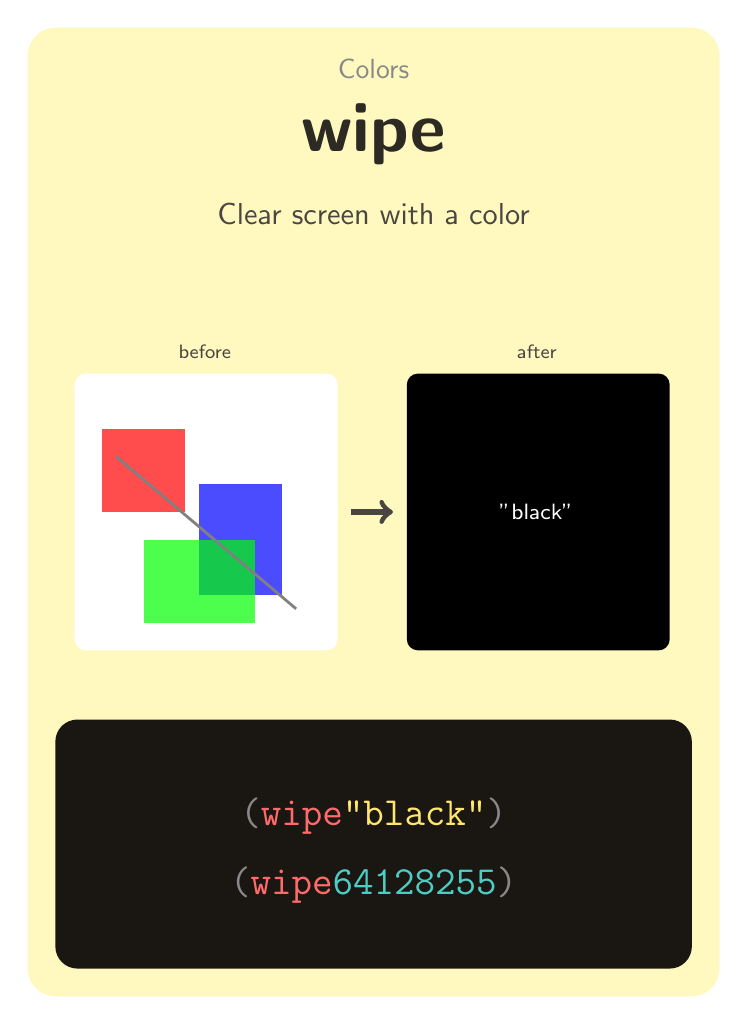
\begin{tikzpicture}
  \fill[cardbg, rounded corners=10pt] (0,0) rectangle (\cardwidth, \cardheight);
  
  \node[anchor=north, font=\sffamily\fontsize{10}{12}\selectfont\color{categorycolor}] 
    at (0.5*\cardwidth, \cardheight-8pt) {Colors};
  
  \node[anchor=north, font=\sffamily\bfseries\fontsize{28}{32}\selectfont\color{titlecolor}] 
    at (0.5*\cardwidth, \cardheight-24pt) {wipe};
  
  \node[anchor=north, text width=\cardwidth-24pt, font=\sffamily\fontsize{11}{14}\selectfont\color{bodycolor}, align=center] 
    at (0.5*\cardwidth, \cardheight-60pt) {Clear screen with a color};
  
  % === VISUAL DIAGRAM - Before/After ===
  \begin{scope}[shift={(12pt, 115pt)}]
    \def\diagramwidth{226pt}
    \def\diagramheight{120pt}
    
    % "Before" - messy screen
    \fill[white, rounded corners=4pt] (5pt, 10pt) rectangle (100pt, 110pt);
    \fill[red, opacity=0.7] (15pt, 60pt) rectangle (45pt, 90pt);
    \fill[blue, opacity=0.7] (50pt, 30pt) rectangle (80pt, 70pt);
    \fill[green, opacity=0.7] (30pt, 20pt) rectangle (70pt, 50pt);
    \draw[gray, line width=1pt] (20pt, 80pt) -- (85pt, 25pt);
    \node[anchor=south, font=\sffamily\fontsize{7}{9}\selectfont\color{bodycolor}] at (52pt, 112pt) {before};
    
    % Arrow
    \draw[->, line width=2pt, bodycolor] (105pt, 60pt) -- (120pt, 60pt);
    
    % "After" - clean black screen
    \fill[black, rounded corners=4pt] (125pt, 10pt) rectangle (220pt, 110pt);
    \node[anchor=south, font=\sffamily\fontsize{7}{9}\selectfont\color{bodycolor}] at (172pt, 112pt) {after};
    \node[anchor=center, font=\sffamily\fontsize{8}{10}\selectfont\color{white}] at (172pt, 60pt) {"black"};
  \end{scope}
  
  % === CODE BLOCK ===
  \fill[codebg, rounded corners=8pt] (10pt, 10pt) rectangle (\cardwidth-10pt, 100pt);
  
  \node[anchor=center] at (0.5*\cardwidth, 65pt) {
    {\fontsize{14}{18}\selectfont\ttfamily
      \textcolor{klparen}{(}%
      \textcolor{klfunction}{wipe}%
      \textcolor{white}{ }%
      \textcolor{klstring}{"black"}%
      \textcolor{klparen}{)}%
    }
  };
  
  \node[anchor=center] at (0.5*\cardwidth, 40pt) {
    {\fontsize{14}{18}\selectfont\ttfamily
      \textcolor{klparen}{(}%
      \textcolor{klfunction}{wipe}%
      \textcolor{white}{ }%
      \textcolor{klnumber}{64}%
      \textcolor{white}{ }%
      \textcolor{klnumber}{128}%
      \textcolor{white}{ }%
      \textcolor{klnumber}{255}%
      \textcolor{klparen}{)}%
    }
  };
\end{tikzpicture}
\end{document}
